\fancyhead[LO, RE]{Obtenir une version propre et finalisée du texte}

\section{Quelles corrections du texte ?}
Notre objectif est de procéder à une analyse des chapitres du Beccaria, et notamment observer le lexique utilisé et les termes juridiques qui ont été employés pour mener à la création du dictionnaire métalexicographique. Ainsi, si nous avons écrit un script pour permettre de mettre en forme les fichiers textes et alors, avoir une matière plus homogène pour l'analyse, il reste tout de même après cela des modifications à réaliser.

En effet, le texte contient un certain nombre de fautes qui sont dues à de multiples éléments~: erreurs lors de la transcription après océrisation\index{OCR!ocerisation@océrisation}, fautes créées par la mise en forme du texte (mots toujours coupés en deux ou tirets enlevés alors que nécessaires) et surtout des erreurs inhérentes à l'époque d'écriture des textes, tel que le verbe \textit{paraître} qui s'écrit \textit{paroître} ou le mot \textit{temps} qui s'écrit \textit{tems}. Si les deux premières ne posent pas trop de problème et peuvent être facilement corrigées, la dernière a demandé plus de réflexions, pour savoir si, dans le principe d'homogénéisation décidé, certains des verbes, noms et adjectifs présents dans le texte doivent être modernisés. Nous avons décidé de ne pas modifier l'écriture des mots dans un souci d'authenticité du texte, mais de tout de même les extraire, pour les ajouter, par la suite, dans un logiciel de statistiques textuelles (choix de \textsc{txm} pour ce projet), pour leur permettre de reconnaître la forme du verbe si elle leur est inconnue.\pagebreak

Une fois ces réflexions faites et le choix de corrections effectué, nous pouvons commencer à manipuler les fichiers textes à l'aide de plusieurs scripts (quatre sont nécessaires pour avoir une version du texte finalisée) qui changeront le texte typographiquement et orthographiquement, notamment à l'aide d'un module Python spécialisé dans la correction orthographique.

\section{Le module \emph{pyspellchecker}~: une vérification quasi automatique de l'orthographe}
Pour opérer les corrections dans le texte, le choix s'est porté sur un module développé pour Python pour faire de la vérification orthographique \footnote{\emph{Pyspellchecker}~: \url{https://github.com/barrust/pyspellchecker}}. Comme tous les modules Python, il peut s'installer sur l'ordinateur à l'aide d'un \emph{pip install} et donne ensuite accès aux différentes méthodes proposées pour effectuer des corrections.

Le module fonctionne avec de multiples langues (le français, l'allemand, l'anglais, l'espagnol et le portugais sont présents dans le module lors de l'installation) à l'aide d'un dictionnaire de fréquences de mots, qu'il est possible d'améliorer en le complétant avec les mots qu'il n'aurait pas reconnu lors de l'utilisation ou même en ajoutant une nouvelle langue à l'aide d'un dictionnaire de mots d'une autre langue qui est exporté et rattaché au module.

Ensuite, en se basant sur ces dictionnaires, le module a la possibilité d'afficher plusieurs types d'informations. Tout d'abord, en lui soumettant un texte, il peut, à l'aide de la méthode \emph{.unknown()} afficher les mots erronés qu'il a trouvé dans le texte et ensuite, nous obtenir par exemple des corrections de deux manières~:
\begin{itemize}
    \item \emph{spell.correction()} --> cela fera apparaître la correction que le vérificateur orthographique considère la plus appropriée~;
    \item \emph{spell.candidates()} --> le vérificateur orthographique présentera les solutions qu'il considère les plus proches du mot erroné.
\end{itemize}
D'autres éléments sont à disposition avec ce module, tel que l'inverse de la méthode \emph{.unknown()}, soit \emph{.known()} qui fait apparaître dans une liste les mots que le dictionnaire a reconnu dans le texte. Nous pouvons également lui demander la fréquence d'un mot choisi à l'aide de \emph{.word\_probability()}, ce qui permettrait par exemple d'en apprendre un peu plus sur le contenu des dictionnaires de fréquences.
Le module de vérification orthographique propose donc de multiples moyens de corriger un texte, en faisant apparaître des informations différentes en fonction de nos recherches et nous avons donc utilisé certaines de ces méthodes, mêlées à des boucles, pour pouvoir effectuer nos corrections de texte.

\section{Opérer des modifications dans le chapitre~: une intervention en plusieurs étapes}
Une fois que sont établies les corrections à réaliser et ce qui sera utilisé pour le faire, nous pouvons mettre en place le processus pour modifier les chapitres et obtenir nos versions finalisées qui seront utilisées pour l'analyse.
\begin{figure}[H]
    \centering
    \fbox{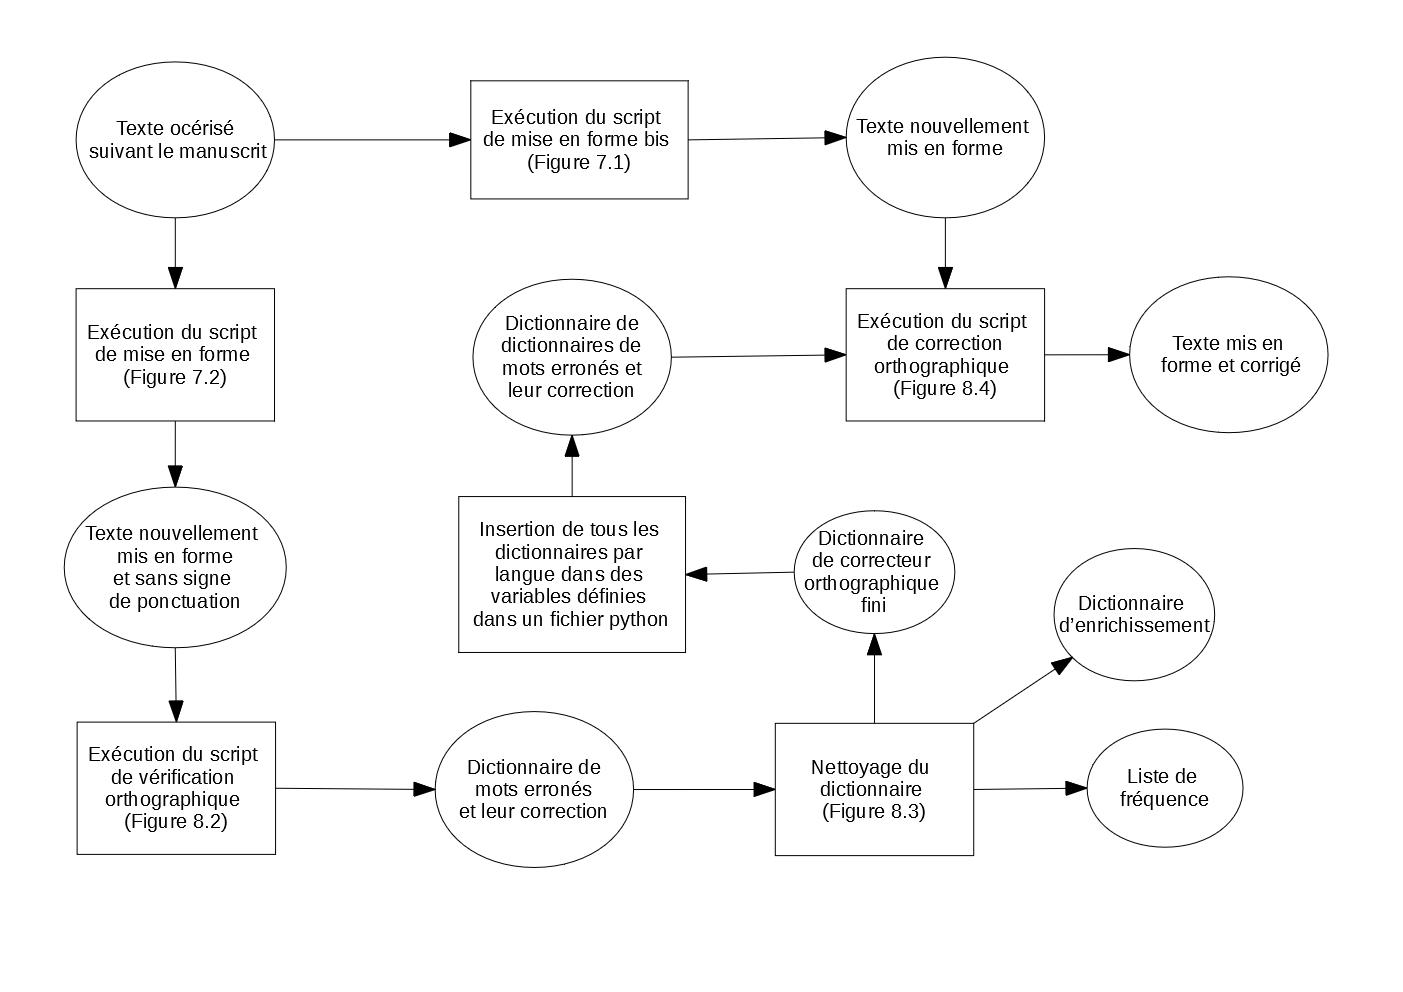
\includegraphics[width=16cm]{Partie2/schemas/Etapes_pour_la_finalisation.jpg}}
    \caption{Diagramme d'activité représentant les étapes pour atteindre une version finalisée et analysable du texte}
    \label{fig:etapestotales}
\end{figure}
Ce diagramme montre le processus qui permettra de partir du texte océrisé de la transcription exacte du manuscrit et d'obtenir une version uniformisée pour permettre une analyse textuelle. Le processus ira tout d'abord changer la mise en forme du texte, pour obtenir une version standard, en supprimant également la ponctuation pour donner la possibilité de traiter le texte et de relever les erreurs orthographiques. Ces erreurs seront traités de trois manières~: soit elles seront inscrites dans une liste pour être plus tard ajoutées aux dictionnaires de langue, soit elles seront inscrites dans un dictionnaire pour recenser les versions non usuelles du mot, soit elles seront ajoutées dans un dictionnaire de correcteur orthographique qui sera manipulé en même temps que le texte. Le dictionnaire orthographique contiendra les mots erronés et leur correction et il sera appliqué, à l'aide d'un autre traitement, au texte de base mis en forme mais cette fois-ci avec sa ponctuation, pour obtenir une version finalisée propre, sans erreur orthographique et prête à être analysée.

\subsection{Une première mise en forme du texte pour faciliter le correcteur}
La première étape consiste à appliquer le script de mise en forme créé précédemment (voir figure \ref{fig:etape1}), pour que le module orthographique puisse plus facilement trouver les mots erronés, sans de multiples tirets ou sans des caractères qui pourraient présenter un problème aux modules. Dans ce cas, nous allons également un peu plus loin que le script de mise en forme basique et nous lui faisons supprimer tous les signes de ponctuation. En effet, ces caractères ont tendance à gêner le correcteur, comme l'apostrophe, puisque le correcteur considère un déterminant et un nom rattaché par une apostrophe comme un mot et de ce point de vue, il ne peut pas le reconnaître, d'où l'intérêt de supprimer ces signes. Pour le cas des points, c'est également nécessaire de les supprimer car lorsqu'une phrase est finie et qu'un point est donc apposé à un mot pour marquer la fin, le correcteur considère le mot avec le point comme une entité et cela l'empêche à nouveau de reconnaître ce qu'il a devant lui. Nous avons donc décidé que pour plus de clarté, il faut supprimer ces éléments-là avant de mettre en fonction le correcteur et de faciliter son application.

\subsection{Éditer le dictionnaire de mots~: trouver les erreurs dans le texte}
La deuxième étape consiste à mettre en application le script de vérification orthographique, pour aller chercher les erreurs du texte pour effectuer plus tard leur correction.
\begin{figure}[t]
    \centering
    \caption{Diagramme d'activité représentant le fonctionnement de la vérification orthographique}
    \fbox{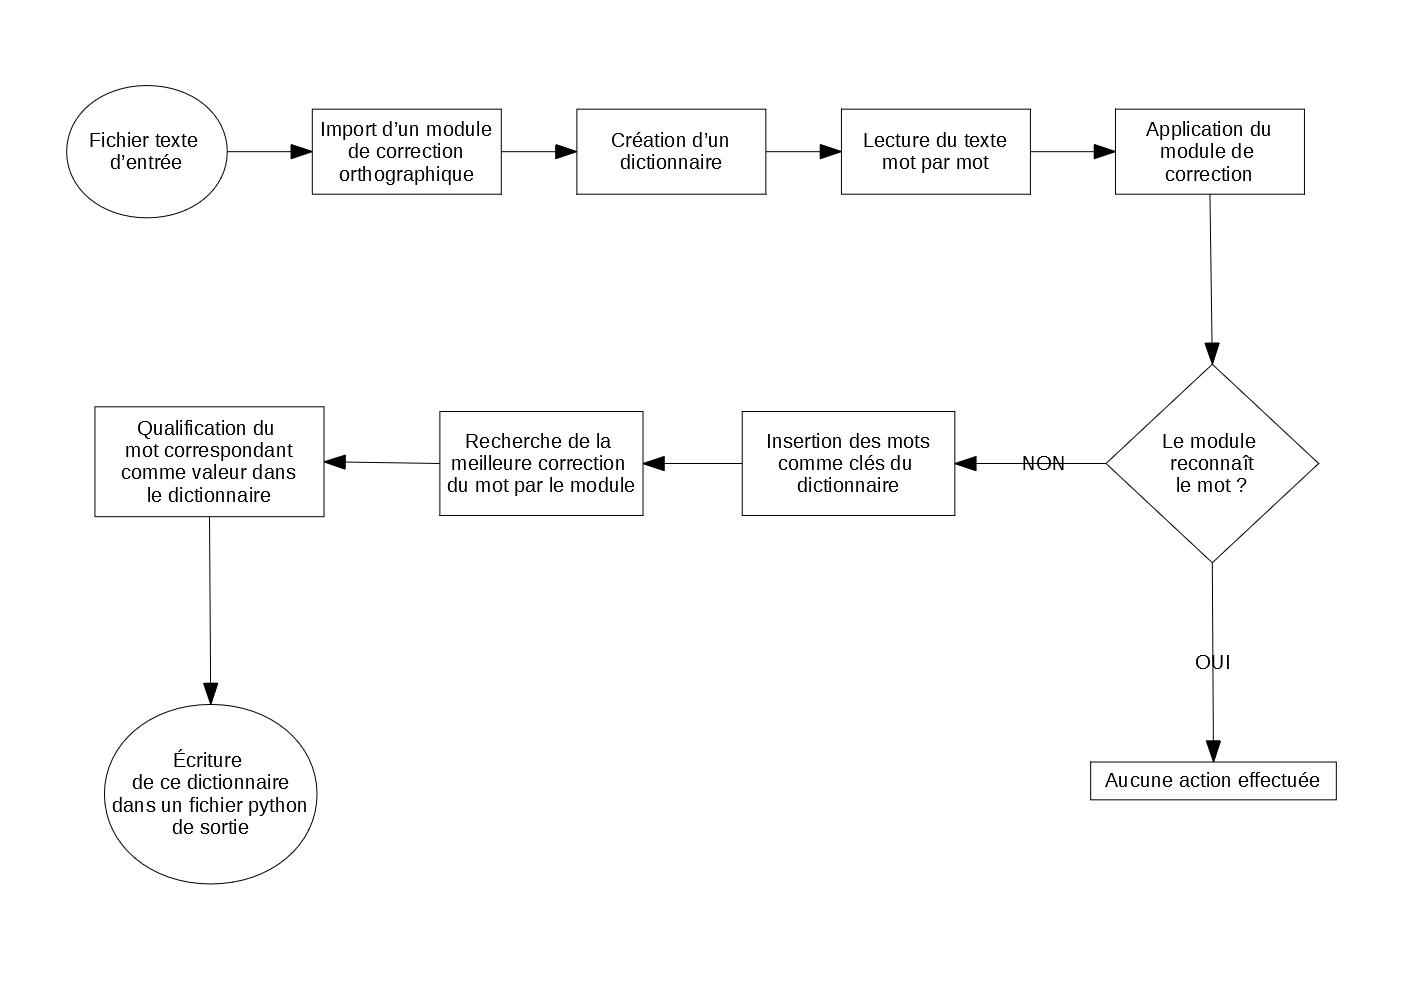
\includegraphics[width=14cm]{Partie2/schemas/2_module_orthographique.jpg}}
    \label{fig:etape2}
\end{figure}
Le processus se déroule comme montré dans la figure \ref{fig:etape2}~: à l'aide d'un module de correction orthographique, un fichier texte sera lu et le module cherchera s'il connaît ou non le mot. Lorsqu'il ne le reconnaîtra pas, ce mot sera inséré dans un fichier extérieur et le module cherchera sa correction la plus probable et lui assignera, créant ainsi un fichier de dictionnaire de mots, utilisable ultérieurement.

En effet, ce script aura pour but de créer un dictionnaire de mots que nous utiliserons ensuite pour corriger le texte mis en forme. Il est établi à l'aide d'une boucle \textit{for} et il consiste à aller chercher dans le texte les mots que le dictionnaire de fréquences de mots ne reconnaît pas. À partir de là, ces mots sont transformés en clés pour le dictionnaire et la valeur de chacune de ces clés est définie comme étant la correction la plus appropriée que conseille le module \emph{pyspellchecker}. Nous obtenons alors un dictionnaire dans un fichier Python qui correspondra à ceci~: \mint{python}{dico = {"mot erroné": "correction proposée"}}

\subsection{Une seconde mise en forme du texte pour rétablir certains éléments}
Une fois la manipulation faite avec le module, le script de mise en forme est de nouveau appliqué, cette fois-ci sans la fonction \og~supprimer\_ponctuation~\fg{}, puisque l'objectif maintenant sera d'avoir un fichier valide, lisible et cohérent et ces éléments-là en sont essentiels (voir figure \ref{fig:etape3}). L'extraction des mots erronés étant faite, nous pouvons récupérer le texte comme nous souhaitions le voir dans le cadre de la réelle mise en forme.

\subsection{Travail sur trois tâches en simultané}
La quatrième étape est probablement la plus rigoureuse de toutes, puisque nous devrons effectuer des changements à la main et au plus proche du texte, pour rendre le travail du correcteur orthographique le plus parfait possible et avoir finalement un document prêt pour une analyse approfondie. Cette étape consiste à la correction du dictionnaire de mots créé deux étapes plus tôt. Nous observons les mots et corrections proposées dans le dictionnaire, pour effectuer quelques modifications si nécessaires pour une correction efficace et cela mène à la réalisation de trois tâches autres mais liées entre elles.
\begin{figure}[H]
    \centering
    \fbox{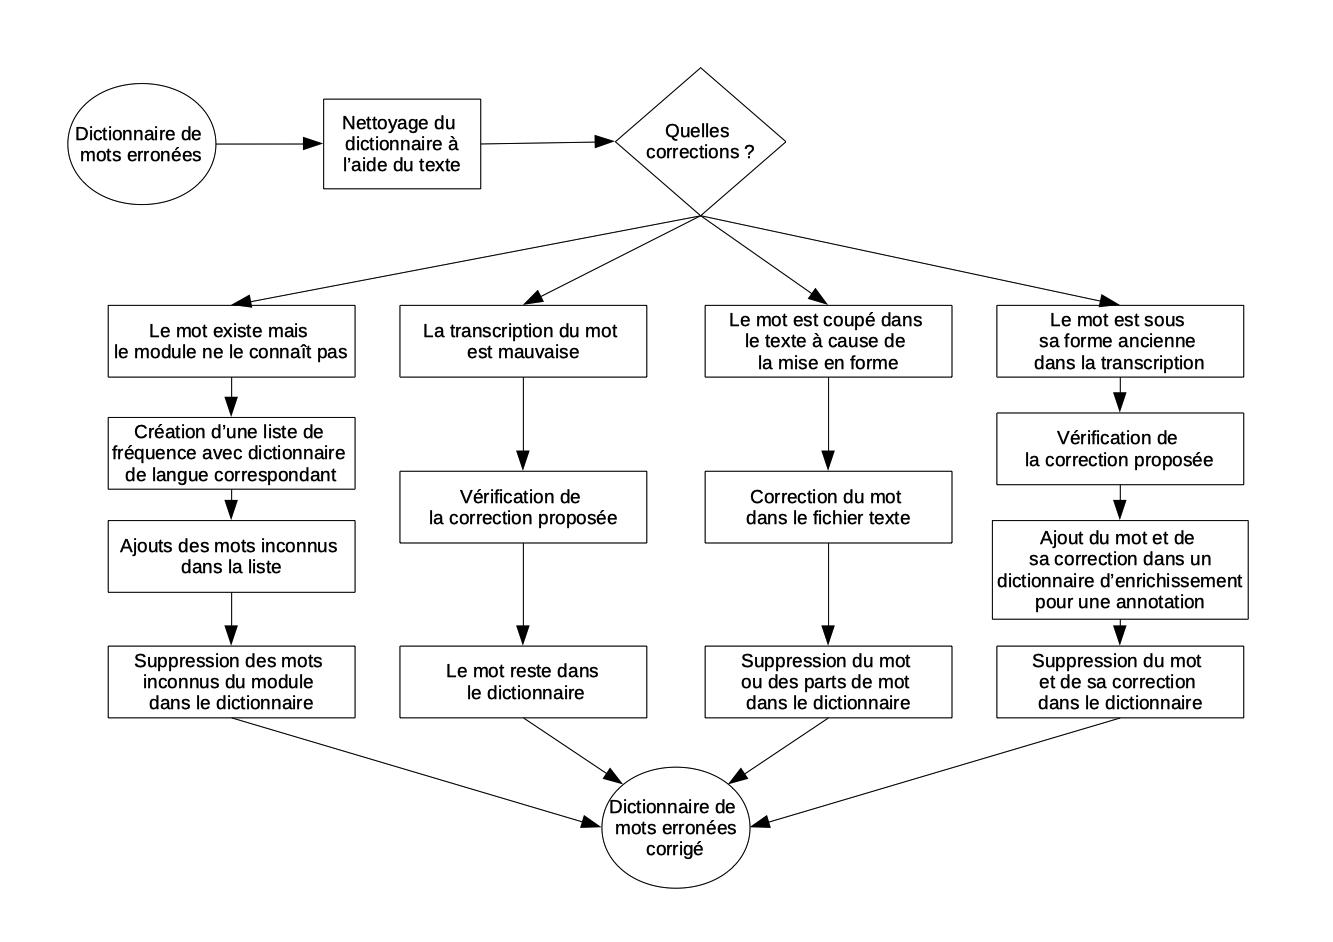
\includegraphics[width=15cm]{Partie2/schemas/4_nettoyage_dico.jpg}}
    \caption{Diagramme d'activité montrant les différentes actions qui permettent le nettoyage du dictionnaire de mots}
    \label{fig:etape4}
\end{figure}
Le dictionnaire de mots erronés nécessite un nettoyage qui s'effectuera à l'aide de quatre actions différentes~: soit le mot existe mais n'est pas connu par le module et il est ajouté à l'aide d'une liste de fréquence, soit le mot est mal transcrit dans le texte et sa correction est laissée ainsi dans le dictionnaire, soit la nouvelle mise en forme du texte a créé des erreurs dans l'écriture du mot et cela est corrigé à même le texte, soit le mot est sous une forme ancienne et il est ajouté dans un dictionnaire d'enrichissement. Une fois cela fait, le résultat est un dictionnaire de mots erronés et leur correction applicable au texte.

\subsubsection{Créer et développer la liste de fréquences}
Tout d'abord, nous observons les mots proposés comme erronés dans le texte par le correcteur orthographique et il arrive à plusieurs reprises que le mot existe et correspond exactement à ce que voulait dire l'auteur mais que le module Python ne le connaisse pas. Dans ce cas-là, ces mots sont supprimés du dictionnaire puisqu'ils doivent être conservés ainsi dans le texte. Ils sont ensuite intégrés dans un script Python qui contiendra une liste de mots qui seront ajoutés dans le dictionnaire de fréquences en fonction de la langue sélectionnée. Cela peut concerner des mots qu'il ne connaît pas, des versions plurielles et féminines du mot ou des conjugaisons qui lui sont inconnues.

\subsubsection{Opérer des changements directs dans le fichier texte}
Si le correcteur trouve des mots qu'il ne connaît pas et qui lui sont rajoutés avec la liste de fréquences, il trouve aussi parfois des erreurs qui vont nécessiter de corriger directement le texte, car cela ne serait pas pratique de le faire avec le script de correction orthographique. Ces modifications expliquent que la deuxième mise en forme se fasse à l'étape précédente, puisqu'il est nécessaire que le texte soit correctement présenté pour ensuite y faire des modifications.

Ainsi, il arrive que des erreurs apparaissent, notamment dues à la séparation par tirets qui existait dans la version originale de la transcription. Le script de mise en forme n'a pas complètement rattaché le mot, ce qui apparaît comme une erreur, que nous corrigerons directement dans le texte, plutôt que de laisser le correcteur le faire. Il faut aussi à l'inverse remettre parfois des tirets, lorsque le mot était composé mais qu'il avait été séparé à une fin de ligne. Ce sont des changements mineurs de vérification du texte transformé mais qui permettent un traitement exhaustif du document.

\subsubsection{Créer un dictionnaire d'enrichissement}
Nos textes de Beccaria ont été édités environ entre 1760 et 1800. A l'époque donc, pour certaines des langues, l'écriture se faisait dans ce qui s'appelle aujourd'hui une langue désuète (ancien français ou autre) avec des versions de certains mots (noms, verbes et leurs conjugaisons) qui ne sont pas les mêmes qu'aujourd'hui. Si nous avons décidé de conserver cela pour nos analyses de texte, il est cependant nécessaire de relever ces mots. Le module le fera logiquement puisque ces formes n'existent pas dans sa base de données. Nous les extrairons à notre tour du dictionnaire de correction et les insérerons dans un dictionnaire d'enrichissement qui servira par la suite à ajouter ces mots à nos modules d'analyses textuelles et notamment \textsc{txm}, pour qu'ils reconnaissent la forme lorsqu'il étudie nos textes.

\subsection{Application du dictionnaire de corrections sur le texte pour obtenir une version finalisée}
Après le travail sur le texte et sur le dictionnaire terminé, nous pouvons passer à la dernière étape, c'est-à-dire apporter les corrections insérées dans le dictionnaire au fichier texte, à l'aide d'un autre script Python.  Après avoir fait les dictionnaires pour chacune des éditions du Beccaria dans une même langue, ils sont tous placés dans un même fichier Python avec une variable donnée à chaque fois (généralement le nom de l'édition auquel il appartient en respectant le sigle défini). Ce fichier de dictionnaires sera par la suite appelé dans le script Python qui est utilisé pour la correction, à l'aide d'une variable.
\begin{figure}[H]
    \centering
    \fbox{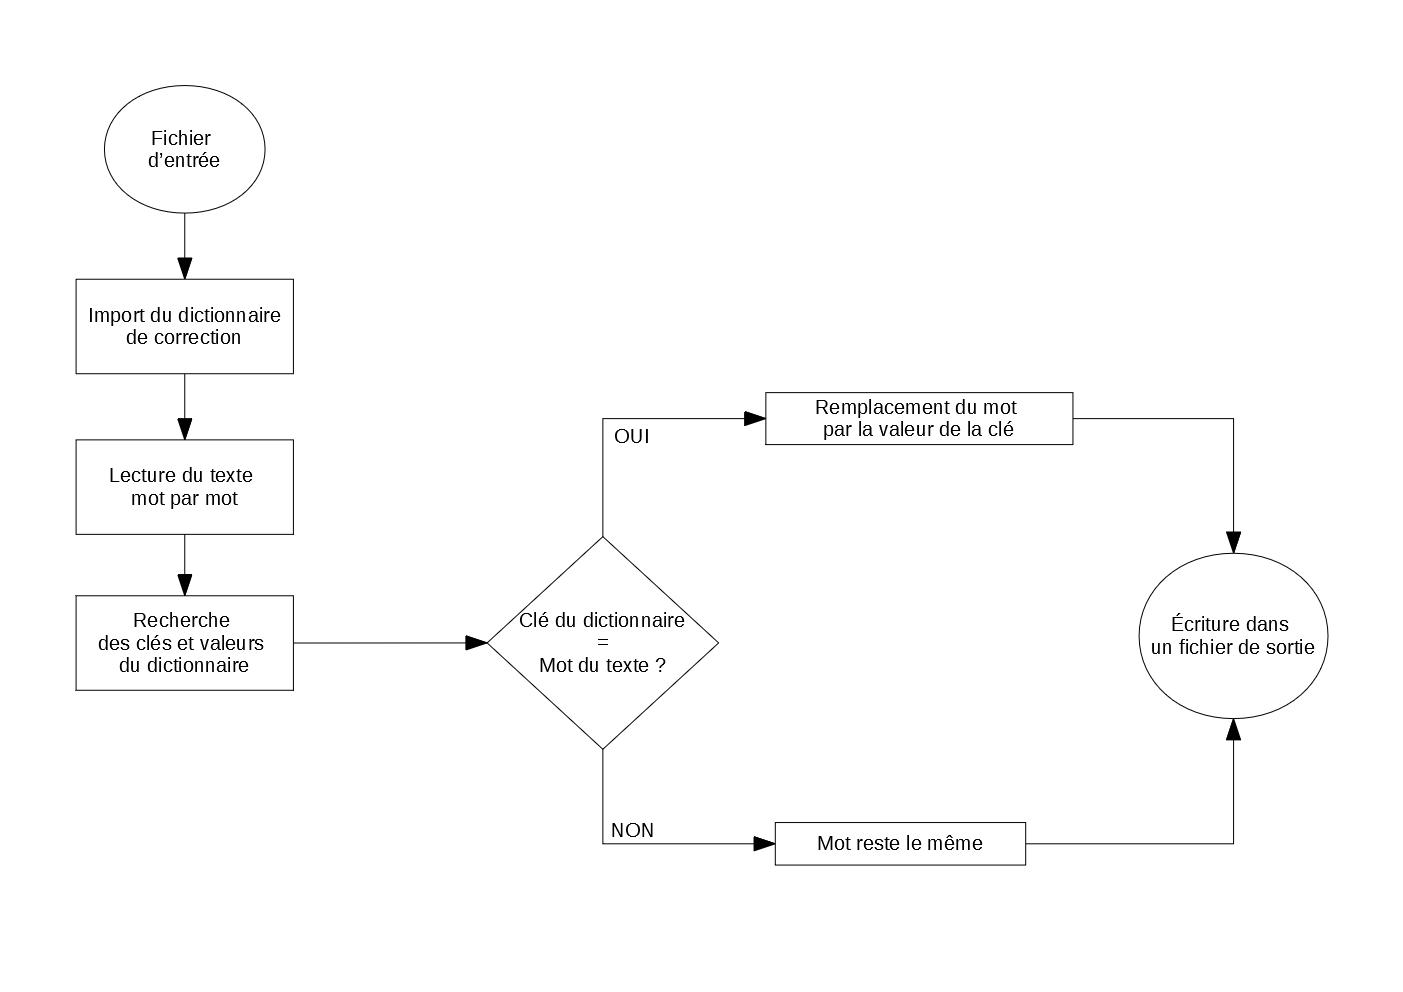
\includegraphics[width=15cm]{Partie2/schemas/5_correction.jpg}}
    \caption{Diagramme d'activité présentant la méthode d'application des corrections orthographiques}
    \label{fig:etape5}
\end{figure}
Le processus consistera à appeler le dictionnaire de mots qui a été traité précédemment et de faire chercher dans le texte les mots qui le composent. Si un mot correspond à un trouvé dans le dictionnaire, le traitement consistera à échanger ce mot par la valeur trouvée dans le dictionnaire, obtenant ainsi une version correcte et propre du texte.

\paragraph{} Le script Python correspondant consiste en une boucle \textit{for} qui sera liée au texte donné et au dictionnaire mis en variable. Il se base sur les clés et les valeurs de ce dictionnaire et il doit simplement aller lire le texte mot à mot, et dans le cas où il trouve un des mots qui font partis des clés de dictionnaires (\mintinline[breaklines]{python}{if cle in texte:}), il doit remplacer ce mot par la valeur de la clé dans le dictionnaire (\mintinline[breaklines]{python}{texte = texte.replace(cle, valeur)}). Ainsi, tous les mots relevés erronés dans le texte seront corrigés et nous obtenons un fichier texte correct orthographiquement, pratique pour l'analyse qui suivra.

\section{Les améliorations à apporter sur le module de correcteur orthographique}
Les différents scripts Python créés fonctionnent aussi bien que souhaité et ils s'adaptent bien au travail que doit réaliser le module \emph{pyspellchecker} mais il est tout de même possible de souligner certains changements à appliquer à l'un ou à l'autre pour une plus grande efficacité dans la correction et pour une meilleure utilisation.

\subsection{Apporter des éléments aux dictionnaires présents~: les listes de fréquences}
Le dictionnaire de mots qui est fourni dans le module de vérificateur orthographique n'est pas exhaustif, comme cela s'observe dans la figure \ref{fig:etape4}, puisqu'il lui arrive d'indiquer certains mots du texte comme faux, alors que ce n'est pas le cas. Lorsque ces cas se présentent, nous mettons en place une liste de fréquence (présente pour chacune des langues travaillées), ce qui fait partie des options proposées par le module \emph{pyspellchecker}.

En effet, dans un souci d'amélioration constante du module et d'application à son propre travail, il est possible d'ajouter des informations dans les dictionnaires avec lesquels nous travaillons. Ainsi, nous pouvons soit mettre un texte entier où tous les mots seront lus et analysés pour être ajoutés ensuite dans le dictionnaire, soit proposer une liste de mots dans le dictionnaire (la méthode choisie), soit n'ajouter qu'un seul mot. Il est également possible d'en supprimer du dictionnaire par la suite.

Alors, en prenant en compte cela, nous avons décidé de créer une liste de fréquences pour chacune des langues, complétée par de nouveaux mots à chaque nouvelle édition d'un dictionnaire depuis un fichier texte et qui s'ajoute au dictionnaire de langue fourni par le module, à chaque fin de travail sur un chapitre particulier.

\subsection{Importer un nouveau dictionnaire de langue~: l'exemple de l'italien}
Pour notre travail sur le traité\index{Traite des delits et des peines@Traité des délits et des peines} de Beccaria, nous étudions des éditions en quatre langues distinctes, dont notamment l'italien, langue d'origine de l'auteur. Cependant, cela a posé problème avec notre module de vérificateur orthographique, puisque cela ne fait pas partie des langues à sa disposition. Il a donc fallu trouver un moyen d'obtenir l'italien pour pouvoir faire une correction de tous les textes à disposition et d'avoir ainsi tous les éléments nécessaires pour l'analyse qui viendra après.

Pour se faire, je suis allée chercher sur le Github qui contient toutes les informations à propos de \emph{pyspellchecker}. Les \emph{issues} du Github m'ont permis de trouver la solution à ce problème, puisque l'une des questions posées était sur l'ajout d'une nouvelle langue dans le module et les moyens utilisés pour le faire \footnote{How to add a new langage \#26~: \url{https://github.com/barrust/pyspellchecker/issues/26}}. L'\textit{issue} renvoie à un autre compte Github qui contient de nombreuses langues avec des listes de fréquences de mots \footnote{FrequencyWords~: \url{https://github.com/hermitdave/FrequencyWords}}, dont notamment l'italien \footnote{\url{https://github.com/hermitdave/FrequencyWords/tree/master/content/2018/it}}. Nous avons donc pu extraire cette liste de mots, la transformer en un dictionnaire de langue, à l'aide d'un script, où le mot correspond à la clé et la fréquence correspond à la valeur et effectuer quelques modifications pour que le fichier soit valide. Une fois cela fait, en suivant les étapes mentionnées dans l'\textit{issue}, nous avons pu insérer le dictionnaire dans le script de vérificateur orthographique utilisé selon la figure \ref{fig:etape2} et ainsi, corriger également les éditions italiennes.

\subsection{Mise en place de lignes de commandes pour l'application du correcteur orthographique}
Enfin, l'une des dernières améliorations concerne moins le module orthographique que son application, et notamment un moyen de simplifier cette application. Le procédé pour corriger le texte contient tout de même quatre à cinq étapes, réalisées pour quatre langues différentes et il est donc nécessaire d'automatiser un minimum ces actions pour gagner du temps et réaliser plus rapidement ces changements.

Nous mettons ainsi en place des scripts shell qui vont contenir les lignes de commande liées au différentes étapes, que nous n'aurons qu'à entrer dans le terminal pour qu'il effectue en une fois tous les changements voulus, tout en respectant cependant chacune des étapes. Ces scripts, identifiés par une extension \emph{.sh}, commencent tous par une ligne unique, essentiel pour définir le fichier comme un script shell, soit \og\#!/bin/bash~\fg{}. Ensuite, sont écrites les informations nécessaires à l'application de nos scripts. Les scripts des trois premières étapes sont très similaires, puisque le changement concerne principalement les chemins des fichiers d'entrées et de sorties et il y a sinon une ligne pour chacune des langues. La quatrième étape est manuelle et donc ne nécessite pas de script. Ce sera pour la cinquième et dernière étape que la création de ces fichiers est la plus nécessaire, puisque là où précédemment, une ligne de commande suffisait pour un dossier complet contenant tous les fichiers d'une même langue, cela n'est pas possible pour la dernière étape. Il est en effet essentiel de préciser pour chacune des éditions le nom du fichier d'entrée et de sortie mais surtout la variable que le script devra aller chercher dans le dictionnaire importé, pour corriger correctement nos documents. Cela équivaut à six à huit lignes de commande, en fonction du nombre d'éditions, ce qui prendrait beaucoup de place et de temps à faire individuellement dans le terminal. Il est donc nécessaire de créer un fichier de ligne de commande pour chacune des langues et de changer le script à chaque nouvelle langue pour appeler le dictionnaire.

Par conséquent, grâce à cette méthode, l'application de notre correcteur orthographique est simplifiée, ce qui permet de corriger plus rapidement et plus efficacement nos fichiers texte, permettant ainsi de procéder plus rapidement au véritable travail à effectuer sur ces éditions, à savoir l'analyse et l'alignement\index{Alignement} des textes.